\documentclass[11pt,a4paper]{article}
\usepackage[margin=25mm]{geometry}
\usepackage{amsmath,amssymb,amsthm,mathtools,booktabs,tikz,hyperref}
\usepackage{microtype}
\hypersetup{hypertexnames=false}
\usepackage{xurl}
\emergencystretch=1em
\usepackage{mathrsfs,tikz-cd}
\providecommand{\tightlist}{\setlength{\itemsep}{0pt}\setlength{\parskip}{0pt}}
\usetikzlibrary{arrows.meta,positioning}
\newtheorem{theorem}{Theorem}[section]
\newtheorem{proposition}[theorem]{Proposition}
\newtheorem{lemma}[theorem]{Lemma}
\theoremstyle{definition}\newtheorem{definition}[theorem]{Definition}
\newtheorem{remark}[theorem]{Remark}
\newcommand{\Z}{\mathbb Z}\newcommand{\Q}{\mathbb Q}
\newcommand{\C}{\mathbb C}\newcommand{\R}{\mathbb R}
\newcommand{\B}{\mathbb B}\newcommand{\N}{\mathbb N}
\newcommand{\F}{\mathbb F}
\newcommand{\Spec}{\operatorname{Spec}}\newcommand{\SpecMon}{\operatorname{Spec}_{\mathrm{mon}}}
\newcommand{\SpecLat}{\operatorname{Spec}_{\mathrm{lat}}}
\newcommand{\supp}{\operatorname{supp}}\newcommand{\tr}{\operatorname{tr}}
\newcommand{\Sch}{\mathcal S}\newcommand{\im}{\operatorname{im}}
\newcommand{\rk}{\operatorname{rank}}\newcommand{\cl}{\operatorname{cl}}
\newcommand{\Pp}{\mathcal P}\newcommand{\LL}{\mathcal L}
\newcommand{\G}{\mathsf G}\newcommand{\Tor}{\operatorname{Tor}}\newcommand{\Frac}{\operatorname{Frac}}
\newcommand{\RZ}{\operatorname{RZ}}\newcommand{\Ann}{\operatorname{Ann}}
\newtheorem{corollary}[theorem]{Corollary}

\providecommand{\Cone}{\operatorname{Cone}}
\providecommand{\Hom}{\operatorname{Hom}}
\providecommand{\Ext}{\operatorname{Ext}}
\providecommand{\RHom}{\operatorname{RHom}}
\providecommand{\coker}{\operatorname{coker}}
\providecommand{\Sh}{\operatorname{Sh}}
\providecommand{\Ab}{\operatorname{Ab}}
\providecommand{\length}{\operatorname{length}}
\providecommand{\PP}{\mathcal P}

\providecommand{\RQ}{\mathbb Q}
\providecommand{\Down}{\operatorname{Down}}

\providecommand{\Dom}{\operatorname{Dom}}
\providecommand{\aug}{\operatorname{aug}}
\providecommand{\Tr}{\operatorname{Tr}}
\providecommand{\Res}{\operatorname{Res}}
\providecommand{\rem}{\operatorname{rem}}
\providecommand{\perm}{\operatorname{perm}}
\providecommand{\sgn}{\operatorname{sgn}}
\providecommand{\pdet}{\operatorname{pdet}}

\providecommand{\Ht}{\mathcal H}
\providecommand{\M}{\mathcal M}
\renewcommand{\Sh}{\mathcal S}
\title{Original Heat Monodromy and Supported Trace Responses}
\author{Split-Zero research programme}
\date{23 September 2026}
\emergencystretch=3em
\errorcontextlines=100
\allowdisplaybreaks


\begin{document}
\maketitle
This continuation evaluates the actual heat-collision monodromy on the
original integral coefficient lattice. It computes each nilpotent
layer's first heat response, retains the complete support lattice in
the resulting parity projections, and applies the same exact
projection construction to the supplied positive eight-state
collision algebra. It uses the actual original heat equation and
all of its analytic coefficients.

The complete predecessor proofs are published as
\href{https://github.com/KokunoYumeto/zeta-function-research-reader/blob/3c022a0adde0a6aa3d8fc8e43ef42795d88e44b0/workbenches/splitzero-tandem/continuations/20260923-supported-zero-collision-holonomy/HEAT_COLLISION_CONDUCTOR.tex}{HC1--30, original conductor and cotangent maps},
\href{https://github.com/KokunoYumeto/zeta-function-research-reader/blob/3c022a0adde0a6aa3d8fc8e43ef42795d88e44b0/workbenches/splitzero-tandem/continuations/20260923-supported-zero-collision-holonomy/HEAT_COLLISION_HOLONOMY.tex}{HH1--43, full-unit connection and arithmetic trace},
and
\href{https://github.com/KokunoYumeto/zeta-function-research-reader/blob/3c022a0adde0a6aa3d8fc8e43ef42795d88e44b0/workbenches/splitzero-tandem/continuations/20260923-supported-zero-collision-holonomy/PRIME_FIXED_SUPPORT_RECEIVER.tex}{PFH1--7, the original two-prime receiver}.
Their entire standalone LaTeX source is also retained in this
package as \texttt{RETAINED\_HEAT\_COLLISION\_PROOFS.tex}.
The degree bounds, convergence, trace responses and projection
identities of the present continuation have their complete proofs below.
\tableofcontents
\clearpage
% Complete independent proof fragment; requires amsmath, amssymb, hyperref.
% Distinct equation prefix HD. Original HH and HC sources are not modified.
\section{The actual heat equation annihilates the integral monodromy defect}
\label{sec:hd}
\newcounter{hd}\renewcommand{\thehd}{HD\arabic{hd}}
\newcommand{\HD}{\refstepcounter{hd}\par\medskip\noindent\textbf{\thehd.}\ }

\HD\textbf{The original objects and the exact question.}
Retain the original Rodgers--Tao convention
\[
 H_t(Z)=\int_0^\infty e^{tu^2}\Phi(u)\cos(Zu)\,du,\qquad
 H_0(Z)=\tfrac18\xi_{\mathrm R}(\tfrac12+iZ/2),\qquad
 \partial_tH_t=-\partial_Z^2H_t,
 \tag{HD1}\label{hd:heat}
\]
where
$\Phi(u)=\sum_{n\ge1}(2\pi^2n^4e^{9u}-3\pi n^2e^{5u})
e^{-\pi n^2e^{4u}}$ and
$\xi_{\mathrm R}(s)=s(s-1)\pi^{-s/2}\Gamma(s/2)\zeta(s)/2$.
The source is Brad Rodgers and Terence Tao,
\emph{The de Bruijn--Newman constant is non-negative},
\href{https://arxiv.org/abs/1801.05914v5}{arXiv:1801.05914v5},
original author equations \texttt{hoz}, \texttt{sas},
\texttt{phidef}, \texttt{htdef} and the following heat-equation sentence.
Fix an actual real zero $x_0$ of $H_0$, of its actual order $m\ge1$.
No multiple-zero existence is assumed. Write, in the original coordinate,
\[
 \xi=Z-x_0,\quad H_0(x_0+\xi)=\sum_{n\ge m}a_n\xi^n,\quad
 a_m\ne0,\qquad A_k=\frac{a_{m+k}}{a_m},\quad A_0=1.
 \tag{HD2}
\]
These real coefficients, including $a_m$, are retained throughout.
The double-exponential decay in HD1 permits arbitrary derivatives
on compact complex $(t,Z)$ sets, dominated by
$C(1+u)^N e^{C u^2+Cu-ce^{4u}}$ for $u\ge1$.
This proves joint holomorphy and legitimizes all local Taylor
identities below.

Put $\mathcal O=\mathbb C\{t\}$ and
$\mathcal K=\operatorname{Frac}\mathcal O$.
The exact monic polynomial $W(t,\xi)$ whose roots are this local
cluster gives
\[
 H_t(x_0+\xi)=U(t,\xi)W(t,\xi),\qquad
 A=\mathcal O[\xi]/W,\quad U(0,\xi)=\sum_{k\ge0}a_{m+k}\xi^k .
 \tag{HD3}\label{hd:original}
\]
The entire analytic unit $U$ is retained.
The auxiliary algebra $B$ and the inclusion $\iota:A\hookrightarrow B$
will be constructed explicitly below. On $B$, $S_B$ changes the
sign of each square-root coordinate. HH14 left the finite module
\[
 \mathcal D_M=(A+M_AA)/A\subset B/A,\qquad
 M_A=\iota_{\mathcal K}^{-1}S_B\iota_{\mathcal K}
 \tag{HD4}\label{hd:defect}
\]
without assuming its vanishing. The conclusion proved here is
$M_AA=A$ and $\mathcal D_M=0$ for every actual multiplicity $m$.
It follows from the heat identities for all the original
coefficients, rather than from a general property of finite
normalization or a presumption that holonomy preserves a lattice.

\HD\textbf{The full heat branches and their defining recursion.}
Define the monic polynomials
\[
 P_n(z)=\sum_{j=0}^{\lfloor n/2\rfloor}
      \frac{(-1)^jn!}{j!(n-2j)!}z^{n-2j},\qquad
 \mathcal P_m(t,y)=
      \sum_{j=0}^{\lfloor m/2\rfloor}
       \frac{(-1)^jm!}{j!(m-2j)!}t^jy^{m-2j}.
 \tag{HD5}\label{hd:hermite}
\]
This is exactly the convention
$P_n(z)=H_n^{\mathrm{Hermite}}(z/2)$ of
\href{https://dlmf.nist.gov/18.5.E13}{DLMF 18.5.13},
Chapter 18 by T.H. Koornwinder, R. Wong, R. Koekoek and
R.F. Swarttouw. The finite formulas fix all constants independently.
Their generating series is $e^{zw-w^2}$, giving
$P_n'=nP_{n-1}$,
$P_{n+1}=zP_n-2nP_{n-1}$, and
$2P_n''-zP_n'+nP_n=0$.
Also $P_ne^{-z^2/4}=(-2)^n\partial_z^n e^{-z^2/4}$, so integration
by parts makes $P_n$ orthogonal to each polynomial of smaller
degree for the positive Gaussian weight. If it had fewer than
$n$ real sign-changing roots, multiplication by the product of
their distinct linear factors would give a nonzero function of
constant sign and contradict that orthogonality. Thus its $n$
roots are real and simple.

Let $r_1<\cdots<r_m$ be the roots of $P_m$ and
$\sigma j=m+1-j$. Then $r_{\sigma j}=-r_j$.
The original heat Taylor identity is the convergent equality
\[
 H_{u^2}(x_0+uz)
       =a_mu^m\sum_{k\ge0}A_k u^kP_{m+k}(z),\qquad t=u^2.
 \tag{HD6}\label{hd:fullseries}
\]
Indeed the heat equation gives
$[t^j\xi^\ell]H_t=(-1)^j(\ell+2j)!a_{\ell+2j}/(j!\ell!)$.
Regroup the absolutely convergent Taylor series by $n=2j+\ell$
on a sufficiently small polydisc.
The analytic implicit-function theorem at $(u,z)=(0,r_j)$ gives
all the branches
\[
 \theta_j(u)=u z_j(u),\quad z_j(0)=r_j,\qquad
 \theta_j(-u)=\theta_{\sigma j}(u),\qquad
 \theta_j(\bar u)=\overline{\theta_j(u)} .
 \tag{HD7}
\]
An isolating circle and the argument principle show that these
are precisely the $m$ zeros of the original nearby cluster.
Every difference is $u(r_j-r_k+O(u))$, so they are distinct off
$u=0$. Their product gives $W$ in HD3.
The quotient $H/W$ is jointly analytic by successive holomorphic
division by the branches on the $u$ cover and invariance under
$u\mapsto-u$; its value at $(0,0)$ is $a_m$, proving that it is a unit.

\HD\textbf{A degree bound forced by the heat equation.}
For all integers $k,q\ge0$ there are polynomials $Q_{k,q}(z)$
such that at every root $r$ of $P_m$,
\[
 \frac{P_{m+k}^{(q)}(r)}{P_m'(r)}=Q_{k,q}(r),\qquad
 Q_{0,0}=0,\qquad
 \deg Q_{k,q}\le k+q-1\quad(k+q\ge1).
 \tag{HD8}\label{hd:Qdegree}
\]
Here zero polynomials satisfy every degree upper bound.
They can be constructed without dividing by a polynomial in $r$:
\begin{align}
 Q_{0,1}&=1,&
 Q_{0,q+2}&=\tfrac12\bigl(zQ_{0,q+1}+(q-m)Q_{0,q}\bigr),\notag\\
 Q_{1,q}&=zQ_{0,q}+qQ_{0,q-1}-2Q_{0,q+1},&
 Q_{k+1,q}&=zQ_{k,q}+qQ_{k,q-1}-2(m+k)Q_{k-1,q}\quad(k\ge1).
 \tag{HD9}\label{hd:Qrecursion}
\end{align}
The terms with a negative second index are declared zero.
The first line comes from repeated differentiation of
$2P_m''-zP_m'+mP_m=0$.
The first formula of the second line uses
$P_{m+1}=zP_m-2P_m'$.
The last formula uses the Hermite recurrence and Leibniz' rule.
They prove the asserted root evaluations and the degree bound
by induction. They also show
$Q_{k,q}(-z)=(-1)^{k+q-1}Q_{k,q}(z)$ whenever $k+q\ge1$.

There are consequently polynomials $p_n(z)$, determined recursively
by the original $A_1,\ldots,A_n$, with
\[
 z_j(u)=r_j+\sum_{n\ge1}p_n(r_j)u^n,\qquad
 \deg p_n\le n-1,\qquad
 p_n(-z)=(-1)^{n-1}p_n(z).
 \tag{HD10}\label{hd:pdegree}
\]
These are coefficient identities in the actual convergent implicit
germs; convergence of $p_n(z)$ for unrestricted $z$ is not required.
For an explicit recursion, let $\delta_{n-1}(u,z)=
\sum_{\nu=1}^{n-1}p_\nu(z)u^\nu$. Then
\[
 p_n(z)=-
 \sum_{\substack{0\le k\le n,\ 0\le q\le n-k\\(k,q)\ne(0,1)}}
 \frac{A_kQ_{k,q}(z)}{q!}
      [u^{\,n-k}]\delta_{n-1}(u,z)^q .
 \tag{HD11}\label{hd:precursion}
\]
The convention $\delta^0=1$ includes the term $k=n,q=0$.
To prove it, substitute the previous coefficients into HD6,
Taylor-expand each polynomial at $r_j$, and divide by $P_m'(r_j)$.
The omitted term contributes exactly the unknown $p_n$.
All remaining terms involve only previous coefficients.
A nonzero monomial in $\delta^q$ has indices
$\nu_1+\cdots+\nu_q=n-k$ and degree at most $n-k-q$.
Together with HD8 its total degree is at most $n-1$.
The same count gives parity $n-1$. For $q=0$ the only possible
term is $k=n$, and HD8 gives the same degree and parity.
This proves the induction and every assertion of HD10.

The bound is the crucial extra constraint: the coefficient of
$u^{n+1}$ in an actual root $\theta_j$ is a polynomial of degree
at most $n-1$ in its original leading Hermite root.
It is two degrees below the unrestricted power $r_j^{n+1}$.
Every $A_n$ is allowed its actual value; none has been set to zero.

\HD\textbf{A convergent coordinate built from all actual branches.}
Let $V_r=(r_j^\ell)_{1\le j\le m,\ 0\le\ell<m}$.
Its determinant is the nonzero real Vandermonde product.
Define analytic germs $\beta_\ell(u)$ by the finite, exact system
\[
 \begin{pmatrix}\beta_0(u)\\ \vdots\\ \beta_{m-1}(u)\end{pmatrix}
       =V_r^{-1}
          \begin{pmatrix}\theta_1(u)-ur_1\\
                          \vdots\\\theta_m(u)-ur_m\end{pmatrix}.
 \tag{HD12}\label{hd:finiteinterp}
\]
For each $\ell$ the quotient $\beta_\ell(u)/u^\ell$ is analytic
and even, and has value zero at $u=0$. More precisely,
\[
 \beta_\ell(u)=u^{\ell+2}B_\ell(u^2),\qquad B_\ell\in\mathbb C\{t\}.
 \tag{HD13}\label{hd:divisibility}
\]
For proof, the coefficient of $u^{n+1}$ in HD12 is the coefficient
vector of the degree-less-than-$m$ interpolation polynomial of
$p_n$ at the roots. If $n+1\le\ell$, its degree is at most
$n-1<\ell$, so its $\ell$th coefficient is zero.
There is no $u^0$ or $u^1$ coefficient either.
Thus $\beta_\ell$ vanishes to order at least $\ell+1$.
HD7 implies $\beta_\ell(-u)=(-1)^\ell\beta_\ell(u)$:
substitution $z\mapsto-z$ gives the unique interpolation polynomial
for the permuted data. This improves the order to $\ell+2$.
The remaining even convergent power series is a convergent germ
in $t=u^2$, proving HD13.

We obtain the exact real-coefficient analytic map
\[
 F(t,y)=y+t\sum_{\ell=0}^{m-1}B_\ell(t)y^\ell,\qquad
 F(0,y)=y,\qquad
 F(u^2,ur_j)=\theta_j(u).
 \tag{HD14}\label{hd:F}
\]
For $m\ge2$ its degree in $y$ is less than $m$; for $m=1$ it is
$y+\theta_1(t)$. This convention includes $m=1$ without pretending
that the representative of $y$ in a rank-one quotient is nonzero.
All coefficients of $F$ are convergent, because HD12 is a fixed
finite matrix applied to convergent germs and HD13 removes only
proved powers of $u$. Thus the construction is analytic, not
merely a formal coordinate transformation.

\HD\textbf{The exact algebra isomorphism and the unchanged arithmetic unit.}
Introduce the auxiliary algebra
\[
 A_{\mathrm H}=\mathcal O[y]/\mathcal P_m(t,y),\qquad
 \varphi:A\longrightarrow A_{\mathrm H},\quad \xi\longmapsto F(t,y).
 \tag{HD15}\label{hd:isomorphism}
\]
The map is well-defined: divide the polynomial $W(t,F(t,y))$ by
the monic $\mathcal P_m$. Its remainder has degree less than $m$
and vanishes at all distinct points $y=ur_j$ for $t\ne0$, by HD14.
It is zero there and hence identically zero by analyticity.
Let $T(t)$ be the matrix whose $k$th column is the coefficient
vector of $F(t,y)^k$ modulo $\mathcal P_m$, for $0\le k<m$.
Reduction by a monic polynomial preserves holomorphic coefficients.
At $t=0$, $F(0,y)=y$ and $\mathcal P_m(0,y)=y^m$, so
\[
 T(0)=I_m,\qquad T\in\operatorname{GL}_m(\mathcal O).
 \tag{HD16}\label{hd:T}
\]
It follows that $\varphi$ is an isomorphism of the complete finite
$\mathcal O$ algebras, in their stated original and auxiliary bases.
It is not an assertion that $W$ equals $\mathcal P_m$.

There is also an exact ambient analytic coordinate description.
Since $F_y(0,0)=1$, the analytic inverse-function theorem gives
$y=G(t,\xi)$ with $F(t,G(t,\xi))=\xi$ and $G(t,F(t,y))=y$.
The full factorization reads
\begin{align}
 W(t,F(t,y))&=\mathcal P_m(t,y)V(t,y),& V(0,y)&=1,\notag\\
 H_t(x_0+F(t,y))&=\mathcal U(t,y)\mathcal P_m(t,y),&
 \mathcal U(t,y)&=U(t,F(t,y))V(t,y).
 \tag{HD17}\label{hd:unit}
\end{align}
Here $V$ is the holomorphic quotient and a unit near the origin;
its value at $t=0$ follows by division of $y^m$ by $y^m$.
In particular $\mathcal U(0,y)=\sum_{k\ge0}a_{m+k}y^k$.
The complete original unit, leading coefficient, coordinate,
and all derivatives are present in HD17. The auxiliary polynomial
has acquired an exact isomorphism from the actual algebra; it has
not been substituted for the original arithmetic function.

\HD\textbf{Evaluation of the integral monodromy defect.}
Let $r=\lfloor m/2\rfloor$, $\epsilon=m-2r$, and index positive
Hermite roots by $r_a>0$. Define
\[
 B=\prod_{a=1}^r\mathbb C\{u_a\}\times\mathcal O^\epsilon,\quad
 u_a^2=t,\qquad
 \iota_{\mathrm H}(y)=(r_au_a)_a\times0,\qquad
 \iota=\iota_{\mathrm H}\varphi .
 \tag{HD18}\label{hd:B}
\]
The central component is omitted when $\epsilon=0$.
For $A$, the coordinate values are exactly
$\theta_a(u_a)=F(u_a^2,r_au_a)$ and the central actual branch
$F(t,0)$. Thus $\iota$ is precisely the original branch inclusion.
Its injectivity follows on the punctured disc by distinct evaluations
and then over $\mathcal O$ by freeness.
The sign automorphism $S_B:u_a\mapsto-u_a$ fixes the central factor.
On $A_{\mathrm H}$ it is the regular involution
$S_{\mathrm H}:y\mapsto-y$, since
$\mathcal P_m(t,-y)=(-1)^m\mathcal P_m(t,y)$.
In the auxiliary power basis its matrix is
$P_0=\operatorname{diag}_{0\le k<m}((-1)^k)$.
Consequently
\[
 \boxed{\quad M_A=\varphi^{-1}S_{\mathrm H}\varphi
             =T(t)^{-1}P_0T(t)\in\operatorname{GL}_m(\mathcal O),
 \qquad M_AA=A,\qquad\mathcal D_M=0.\quad}
 \tag{HD19}\label{hd:vanishing}
\]
This agrees with the original parameter holonomy:
both maps exchange the evaluations at $\theta_j(u)$ and
$\theta_{\sigma j}(u)$, so they agree on the etale algebra;
injectivity gives the stated extension on $A$.
Its original special-fibre action is exactly
\[
 M_A(0)(\xi^k)=(-1)^k\xi^k,\qquad
 A/tA=\mathbb C[\xi]/(\xi^m).
 \tag{HD20}\label{hd:central}
\]
Every nilpotent layer is retained. For $m\ge2$ the involution is
nonidentity even though the defect vanishes; for $m=1$ it is
the identity.

In ambient coordinates this involution has the convergent formula
\[
 \Psi(t,\xi)=F(t,-G(t,\xi)),\qquad
 \Psi(t,\Psi(t,\xi))=\xi,\qquad \Psi(0,\xi)=-\xi .
 \tag{HD21}\label{hd:ambient}
\]
It preserves the actual zero divisor with its exact unit:
\[
 H_t(x_0+\Psi(t,\xi))
   =(-1)^m
     \frac{\mathcal U(t,-G(t,\xi))}{\mathcal U(t,G(t,\xi))}
       H_t(x_0+\xi).
 \tag{HD22}\label{hd:fullunit}
\]
This follows by applying HD17 twice and using the parity of
$\mathcal P_m$. The quotient is an analytic unit.
Thus this is a local symmetry of the full original divisor,
with a specified transformation of the original function;
it does not assert that $H_t$ itself has an unweighted reflection
symmetry about the colliding point.

\HD\textbf{The divisibility criterion in the original matrix $J=CD$.}
The previous result also evaluates, entry by entry, the exact
criterion asked for in the original lattice presentation.
For any such branch inclusion write
\[
 J=C(t)D(t),\qquad
 D=\operatorname{diag}(t^{d_k}),\quad d_k=\lfloor k/2\rfloor,
 \qquad K(t)=C(t)^{-1}S_BC(t).
 \tag{HD23}
\]
The matrix $C$ is the entire unit matrix of HC7, not its value at zero.
In its coordinates the defect is
\[
 \mathcal D_M\simeq
 \operatorname{im}\left(
  \mathcal O^m\xrightarrow{\ KD\ }
       \bigoplus_{i=0}^{m-1}\mathcal O/(t^{d_i})\right).
 \tag{HD24}\label{hd:criterion-module}
\]
Indeed $C^{-1}$ sends $J\mathcal O^m$ to $D\mathcal O^m$ and
$S_BJ\mathcal O^m$ to $KD\mathcal O^m$.
It follows that
\[
 M_AA=A
 \ \Longleftrightarrow\
 K_{ik}(t)\in t^{\max(d_i-d_k,0)}\mathcal O
          \quad\hbox{for all }i,k.
 \tag{HD25}\label{hd:criterion}
\]
For necessity and sufficiency, the entries of
$D^{-1}KD$ are $t^{d_k-d_i}K_{ik}$.
Their integrality is exactly the stated criterion; applying the
involution twice makes inclusion equivalent to equality.
Equivalently, every coefficient
$[t^\nu]K_{ik}$ with $0\le\nu<d_i-d_k$ must vanish.

The actual heat equation proves all these conditions simultaneously.
Let $J_{\mathrm H}$ be the inclusion matrix for HD18. Exact evaluation
gives
\[
 J=J_{\mathrm H}T,\qquad
 S_BJ_{\mathrm H}=J_{\mathrm H}P_0,\qquad
 D^{-1}KD=T^{-1}P_0T .
 \tag{HD26}\label{hd:Jidentity}
\]
The right side is integral by HD16; hence every required coefficient
vanishes by a proved identity involving all actual branches.
This evaluates the original defect rather than discarding the
larger quotient $B/A$. That latter quotient, its conductor and
its nilpotent special-fibre map remain those of HC8--13; its length
$\lfloor(m-1)^2/4\rfloor$ can be positive while HD24 is zero.

\HD\textbf{The first arithmetic coefficients and the exact first variation.}
Use the original ratios
\[
 c=A_1,\quad d=A_2,\quad e=A_3,\quad
 b=2d-c^2,\qquad h=e-cd+\frac{c^3}{3}.
 \tag{HD27}
\]
The explicit recursion gives
\[
 p_1=2c,\qquad p_2=bz,\qquad
 p_3=2h\bigl(z^2-2(m+2)\bigr).
 \tag{HD28}\label{hd:firstcoeffs}
\]
For a direct check of the first new even term,
$Q_{0,2}=z/2$,
$Q_{0,3}=z^2/4-(m-1)/2$,
$Q_{1,1}=0$, $Q_{1,2}=m+1$,
$Q_{2,1}=-2(m+2)$ and
$Q_{3,0}=-2z^2+4(m+2)$.
Substitution in HD11 yields respectively the coefficient
$2h$ of $z^2$ and the constant $-4(m+2)h$.
Thus the full branches have
\[
 \theta_j(u)=r_ju+2cu^2+b r_ju^3
             +2h\bigl(r_j^2-2(m+2)\bigr)u^4+O(u^5).
 \tag{HD29}
\]
Every remainder here is from the fixed actual convergent germ.

There is an exact expression for the whole coefficient of $t$,
not just the displayed low powers. Define the original logarithmic
unit coefficients by
\[
 \log\frac{U(0,z)}{a_m}
       =\log\left(1+\sum_{n\ge1}A_nz^n\right)
       =\sum_{n\ge1}\ell_nz^n .
 \tag{HD30}\label{hd:logunit}
\]
This is the unique local logarithm with value zero at zero.
In particular $\ell_1=c$, $\ell_2=d-c^2/2$, $\ell_3=h$, and
\[
 \ell_5=A_5-cA_4-d e+c^2e+cd^2-c^3d+c^5/5.
 \tag{HD31}
\]
For $1\le n\le m$, the coefficient of $z^{n-1}$ in $p_n(z)$
is $2\ell_n$.
Here is a complete coefficient proof. The leading term of
$Q_{0,q}$ for $q\ge1$ is $2^{1-q}z^{q-1}$ by HD9.
The leading term of $Q_{k,0}$ for $k\ge1$ is $-2z^{k-1}$.
For $k,q\ge1$, derivative identities give a representative of degree
at most $k+q-3$: if $q<k$, use
$P_{m+k}^{(q)}=(m+k)!P_{m+k-q}/(m+k-q)!$;
if $q=k$, the value is zero; if $q>k$, use
$P_{m+k}^{(q)}=((m+k)!/m!)P_m^{(q-k)}$.
When $k+q\le n\le m$, this representative and HD9's representative
both have degree less than $m$ and agree at all $m$ roots;
they are therefore the same polynomial. These mixed terms cannot
contribute to degree $n-1$ in HD11 for the stated range.
If $v_n=[z^{n-1}]p_n$ and $V(w)=\sum_{n=1}^m v_nw^n$,
the remaining highest-degree coefficients say exactly
\[
 2\bigl(e^{V(w)/2}-1\bigr)-2\sum_{n=1}^m A_nw^n
          =0\pmod{w^{m+1}}.
 \tag{HD32}
\]
This is an identity of truncated formal coefficient series, so its
unique solution is
$V(w)=2\log(1+\sum A_nw^n)\pmod{w^{m+1}}$.
This proves exactly the coefficients used below, with no
asymptotic argument in $z$ or choice of a polynomial representative
above degree $m-1$.

In HD12--14, a term $t y^{n-1}$ has weight $n+1$ for
$\operatorname{wt}t=2$, $\operatorname{wt}y=1$.
Only the top coefficient of $p_n$ supplies it, and $n-1<m$
means that no interpolation reduction is needed. Hence
\[
 \partial_t F(0,y)=2\sum_{n=1}^m\ell_n y^{n-1},\qquad
 \Psi(t,\xi)=-\xi+
       4t\sum_{\substack{1\le n\le m\\ n\ {\rm odd}}}
                         \ell_n\xi^{n-1}+O(t^2).
 \tag{HD33}\label{hd:firstvariation}
\]
The first equality is an equality of polynomials for the chosen
$F$; it also applies to $m=1$.
The second is an equality of analytic germs in $(t,\xi)$:
differentiate $F(t,-G(t,\xi))$, using
$\partial_tG(0,\xi)=-\partial_tF(0,\xi)$.
Thus the actual unit determines every first-order matrix entry.

For $m\ge2$, in the original basis $1,\xi,\ldots,\xi^{m-1}$,
the first variation is especially explicit. For $1\le k<m$,
\[
 M_A(\xi^k)=(-1)^k\xi^k+
 4k(-1)^{k-1}t
   \sum_{\substack{n\ {\rm odd},\ n\ge1\\k+n-2<m}}
                 \ell_n\,\xi^{k+n-2}+O(t^2A),
 \qquad M_A(1)=1 .
 \tag{HD34}\label{hd:matrixvariation}
\]
Terms already multiplied by $t$ may be reduced modulo $\xi^m$
to this order, since $W(0,\xi)=\xi^m$.
This proves each coefficient and sign in the stated original basis.

\HD\textbf{Multiplicities one and two.}
For $m=1$ there is one analytic branch and $A=B=\mathcal O$.
The action is the identity and the defect is zero.
For $m=2$ there is one quadratic component,
\[
 W=(\xi-E(t))^2-tR(t)^2,\qquad
 M_A(\xi)=2E(t)-\xi,\qquad A=B,\quad\mathcal D_M=0 .
 \tag{HD35}
\]
Here $R(0)=\sqrt2$ and both complete germs are the actual
even and odd branch parts. HD29 evaluates
$E(t)=2ct-12ht^2+O(t^3)$.
The coefficient $-12h$ uses $r_j^2=2$ and $m+2=4$.
Thus $M_A(\xi)=-\xi+4ct-24ht^2+O(t^3)$ exactly in this rank-two
algebra. No unit has been set equal to a constant.

\HD\textbf{Multiplicity three: a nonzero normalization quotient, zero loop defect.}
Write the actual factors as
$Q=(\xi-E(t))^2-tR(t)^2$ and $\xi-\eta(t)$, with $R(0)=\sqrt6$.
All three germs include every higher arithmetic coefficient.
The exact generator image is
\[
 M_A(\xi)=-\xi+2E(t)+2\lambda(t)Q(t,\xi),\qquad
 \lambda(t)=\frac{\eta(t)-E(t)}
                {(\eta(t)-E(t))^2-tR(t)^2}.
 \tag{HD36}\label{hd:m3}
\]
At the two quadratic roots this is $2E-\xi$, and at $\xi=\eta$
it equals $\eta$; injectivity of the full branch evaluations
therefore proves the formula. HD29 gives
\[
 E=2ct-8ht^2+O(t^3),\quad
 \eta=2ct-20ht^2+O(t^3),\quad
 R^2=6(1+2bt)+O(t^2),\quad
 \lambda=2ht+O(t^2).
 \tag{HD37}
\]
In particular the displayed quotient in HD36 is analytic: its
denominator is $t$ times a unit with constant $-6$, and its
numerator has order at least two. This checks directly the first
case with $B/A\simeq\mathcal O/(t)$.
Its entire holonomy matrix begins
\[
 M_A=
 \begin{pmatrix}
  1&4ct&0\\
  0&-1&-8ct\\
  0&4ht&1
 \end{pmatrix}
       +O(t^2),\qquad \mathcal D_M=0 .
 \tag{HD38}
\]
The notation $O(t^2)$ is entrywise and the first column is exactly
$(1,0,0)^T$. The $h$ term is the original coefficient
$a_{m+3}/a_m-cd+c^3/3$, not a freely selected polynomial parameter.

\HD\textbf{Multiplicity four: all two-pair denominators cancel.}
There are two actual quadratic factors
$Q_a=(\xi-E_a)^2-tR_a^2$, with
$r_1^2=6-2\sqrt6$, $r_2^2=6+2\sqrt6$ and $R_a(0)=r_a>0$.
Put, retaining all germs,
\[
 \Delta=E_2-E_1,\quad a=2\Delta,\quad
 b_0=\Delta^2+t(R_2^2-R_1^2),\quad
 \mathfrak r=b_0^2-a^2tR_2^2 .
 \tag{HD39}
\]
Then the exact original-coordinate formula is
\[
 M_A(\xi)=-\xi+2E_1+
     2\Delta Q_1(t,\xi)
       \frac{b_0-a(\xi-E_2)}{\mathfrak r}.
 \tag{HD40}\label{hd:m4}
\]
Indeed modulo $Q_2$,
$Q_1=a(\xi-E_2)+b_0$ and $(\xi-E_2)^2=tR_2^2$.
The fraction is the multiplicative inverse of $Q_1$ modulo $Q_2$.
The added term vanishes modulo $Q_1$ and equals $2\Delta$
modulo $Q_2$, which proves every evaluation in HD40.

HD29 shows $\Delta=2h(r_2^2-r_1^2)t^2+O(t^3)$ and
$b_0=(r_2^2-r_1^2)t+O(t^2)$.
Thus $\mathfrak r=t^2$ times a unit with constant
$(r_2^2-r_1^2)^2=96$. The two coefficient quotients
$\Delta b_0/\mathfrak r$ and $\Delta a/\mathfrak r$ have orders
at least one and two, respectively. This proves analyticity
without cancelling any unspecified arithmetic factor.
Here $B/A\simeq(\mathcal O/(t))^2$, but its loop submodule is zero.
The full matrix has first-order part
\[
 M_A=
 \begin{pmatrix}
 1&4ct&0&0\\
 0&-1&-8ct&0\\
 0&4ht&1&12ct\\
 0&0&-8ht&-1
 \end{pmatrix}
       +O(t^2),\qquad \mathcal D_M=0 .
 \tag{HD41}
\]
Again every higher coefficient is specified by the convergent
original-coordinate formula HD40 or, equivalently, HD19.

\HD\textbf{The next multiplicities and the first additional constraints.}
For $m=5,6$ the largest exponent $d_i$ in HD23 is two, so
$t^2B\subset A$. All actual pair centres and the central branch
have common term $2ct$ by HD29. The even-centre vector is therefore
$2ct\cdot1+t^2b_2$ with $b_2\in B$, and lies in $A$.
The generator image $M_A(\xi)$ is twice this vector minus $\xi$,
which directly proves the criterion in these two cases.
The first new coefficient of its matrix is completely determined:
\[
 M_A(\xi)=-\xi+4t(c+h\xi^2+\ell_5\xi^4)+O(t^2A),
       \qquad m=5\ \hbox{or}\ 6 .
 \tag{HD42}
\]
All entries of the remaining columns are given by HD34.
The coefficient $\ell_5$ is the full arithmetic expression HD31.

For $m=7,8$ one has $t^3B\subset A$. Now the exact fourth-order
root coefficient is needed. The pair-centre vector, including
the central component if present, satisfies
\[
 E_{\mathrm{vec}}=
  2ct\cdot1+
  2ht(\xi-2ct)^2-4(m+2)ht^2\cdot1\pmod{t^3B}.
 \tag{HD43}
\]
To check both kinds of $B$ coordinates, on each pair
$\xi-2ct=r_au_a+b r_au_a^3+O(u_a^4)$.
Its even square is $r_a^2t+O(t^2)$.
Its odd square has order at least $u_a^5$; after division by
$u_a$ and multiplication by $t$ it belongs to $t^3\mathcal O$.
Thus the right side has the required even coefficient
$2ct+2h(r_a^2-2(m+2))t^2$, with zero odd coefficient modulo
$t^3B$. The central coordinate gives
$2ct-4(m+2)ht^2$ as required. This proves HD43.
Every displayed term lies in $A$, so the centre vector does too,
and again $\mathcal D_M=0$.
For all larger multiplicities HD10--19 give the finite, convergent
continuation of these cancellations, rather than a finite-order
presumption about uncomputed terms.

\HD\textbf{Retained fibres and the exact additional receiver.}
The vanishing of HD4 concerns this specific loop-lattice defect.
It does not annihilate $B/A$, its conductor, the cotangent torsion,
or the original trace radical. For example HD20 acts by signs
on all powers in $\mathbb C[\xi]/\xi^m$, while the original
reflected trace at the endpoint remains
$m\overline{f(0)}g(0)$ and has radical $(\xi)$ when $m>1$.
The endpoint $v=i\xi/2$ is the original arithmetic jet coordinate,
and the loop acts by $v\mapsto-v$ there. The arithmetic multiplier
$e^{iLx_0/2}\exp(LM_v)$ remains its separate full operator;
the commutator and trace comparisons proved in HH33--38 apply
to the now established regular lattice automorphism.

For every original bounded distributive support lattice $\Lambda$,
there is now an actual lifted algebra involution
\[
 G_\Lambda(A)\longrightarrow G_\Lambda(A),\qquad
 (a,1_\Lambda)\longmapsto(M_Aa,1_\Lambda),\qquad
 (0,\lambda)\longmapsto(0,\lambda).
 \tag{HD44}
\]
It preserves both operations because $M_A$ is a unital
$\mathcal O$-algebra automorphism and every support coordinate
is fixed. Its square is the identity; its arithmetic projection
is HD19 and its support projection is the identity on the
complete original lattice. This proves the strongest extension
specified by the formerly unevaluated defect.
It supplies no nonreal zero of the original $H_0$ and no negative
test for the complete original Weil form.


\section{The original coefficient flags and the first heat response of the socle}
\label{sec:heat-flag-response}

This calculation starts with the actual heat family, coordinates and
full analytic unit of HC1--4 and HH1--6. Those proofs retain the
Rodgers--Tao convention $H_t(z)=\int_0^\infty e^{tu^2}\Phi(u)\cos(zu)\,du$,
$\partial_tH_t=-\partial_z^2H_t$, and
$H_0(z)=\xi_{\mathrm R}(1/2+iz/2)/8$ from
Brad Rodgers and Terence Tao,
\href{https://arxiv.org/abs/1801.05914v5}{\emph{The de Bruijn--Newman constant is non-negative}},
author equations \texttt{hoz}, \texttt{htdef} and \texttt{sas}.
The original local Weil contribution and its full multiplicity are
identified in HH23--30 using Alain Connes and Caterina Consani,
\href{https://arxiv.org/abs/2207.10419}{\emph{Hochschild homology, trace map and zeta-cycles}},
Proposition \texttt{laplacian} and Remark \texttt{remtauto}, and
\href{https://arxiv.org/abs/2006.13771v1}{\emph{Weil positivity and trace formula, the archimedean place}}.
All finite algebra, limits and coefficients used below are proved here.

Fix an actual real zero $x_0$ of order $m\ge1$. Write $\xi=z-x_0$,
$t=u^2$, and retain the entire original polynomial
$W(t,\xi)=\prod_{\nu=1}^m(\xi-\theta_\nu(u))$ and unit
$H_t(x_0+\xi)=U(t,\xi)W(t,\xi)$. Put
\[
 c=a_{m+1}/a_m,\quad d=a_{m+2}/a_m,\quad b=2d-c^2,
 \qquad
 \theta_\nu(u)=r_\nu u+2cu^2+b r_\nu u^3+O(u^4).
 \tag{HF1}
\]
The $r_\nu$ are all the distinct real roots of
\[
 P_m(y)=\sum_{a=0}^{\lfloor m/2\rfloor}
 \frac{(-1)^a m!}{a!(m-2a)!}y^{m-2a}.
 \tag{HF2}
\]
No multiple zero is asserted to exist. The construction applies to
each actual zero with its actual order. In particular it includes $m=1$.

\paragraph{HF1. The full original trace matrix.}
Let $\mathcal O=\mathbb C\{t\}$,
$A=\mathcal O[\xi]/(W)$ and retain its ordered basis
$1,\xi,\ldots,\xi^{m-1}$. For real $t$, conjugation fixes $t,\xi$;
write $f^\#(\xi)=\overline{f(\bar\xi)}$. The reflected regular trace is
\[
 T_t(f,g)=\operatorname{Tr}_{A_t/\mathbb C}(M_{f^\#g}),
 \qquad K_{ij}(t)=s_{i+j}(t),\qquad
 s_n(t)=\sum_{\nu=1}^m\theta_\nu(u)^n,
 \quad 0\le i,j<m.
 \tag{HF3}
\]
The sum is unchanged by $u\mapsto-u$, which permutes the branches;
it is thus analytic in $t$. At $t\ne0$ the algebra is reduced and
the formula is evaluation of its multiplication trace. At zero it
continues to that same trace by the companion matrix of $W$.
Consequently HF3 is an exact identity at every fibre, including
the nonreduced one, and $K(0)=\operatorname{diag}(m,0,\ldots,0)$.

For $0\le j<m$ define the original coefficient submodule
\[
 F^jA=\operatorname{span}_{\mathcal O}
          \{\xi^j,\xi^{j+1},\ldots,\xi^{m-1}\}.
 \tag{HF4}
\]
These are specified free submodules in the original basis. They
are not silently identified with ideals of all deformed fibres.
Their specializations are the ideals $(\xi^j)$ of
$A_0=\mathbb C[\xi]/(\xi^m)$.

\paragraph{HF2. All successive trace responses are evaluated.}
Put $p_n=\sum_\nu r_\nu^n$, including $p_0=m$. For $f,g\in F^jA$
with coefficient functions $f_k(t),g_k(t)$, the exact limit is
\[
 \boxed{\lim_{t\to0}t^{-j}T_t(f(t),g(t))
       =p_{2j}\,\overline{f_j(0)}g_j(0).}
 \tag{HF5}
\]
Here the limit is along real $t$; the matrix quotient has an analytic
continuation through zero. To prove it, HF1 gives
$s_{2a}(t)=p_{2a}t^a+O(t^{a+1})$, while evenness in $u$ gives
$s_{2a+1}(t)=O(t^{a+1})$. If $i,j\ge j_0$ and
$i+j>2j_0$, then $s_{i+j}(t)=O(t^{j_0+1})$.
The only entry of $t^{-j_0}K|_{F^{j_0}}$ surviving at zero is
therefore $(j_0,j_0)$, with value $p_{2j_0}$. Multiplying by the
analytic coefficient columns proves HF5.

For $j=0$, $p_0=m>0$. For $m\ge2$ and $j>0$, at least one
$r_\nu$ is nonzero, so $p_{2j}>0$. Thus HF5 has radical
$F^{j+1}A_0$ inside $F^jA_0$ and is positive definite on the
one-dimensional quotient $F^jA_0/F^{j+1}A_0$.
Every endpoint nilpotent layer has an explicitly determined
first heat response. This is a statement about the time derivatives
of the retained family, not a new positive value assigned to $T_0$.
In particular,
\[
 \left.\frac d{dt}T_t(f,g)\right|_{t=0}
    =2m(m-1)\,\overline{f_1(0)}g_1(0),
       \qquad f,g\in F^1A.
 \tag{HF6}
\]
The identity $p_2=2m(m-1)$ follows from the coefficient
$-m(m-1)$ of $y^{m-2}$ in HF2 and Newton's second identity.

\paragraph{HF3. The coefficients are finite exact data.}
Writing $P_m(y)=y^m+\alpha_1y^{m-1}+\cdots+\alpha_m$, all
$\alpha_{2a}=(-1)^a m!/(a!(m-2a)!)$ and all odd $\alpha_k$ vanish.
The required $p_n$, including $p_{2m-2}$, are evaluated by
\[
 \begin{cases}
 p_n+\alpha_1p_{n-1}+\cdots+\alpha_{n-1}p_1+n\alpha_n=0,
          &1\le n\le m,\\
 p_n+\alpha_1p_{n-1}+\cdots+\alpha_m p_{n-m}=0,&n>m.
 \end{cases}
 \tag{HF7}
\]
For completeness, expand
$P_m'(y)/P_m(y)=\sum_\nu(y-r_\nu)^{-1}
=\sum_{n\ge0}p_n y^{-n-1}$ at infinity, multiply by $P_m(y)$,
and equate coefficients. This proves HF7 without numerical root
approximation. The Hermite convention in HF2 agrees with
\href{https://dlmf.nist.gov/18.5.E13}{DLMF18.5.13}, Chapter18 by
T.~H. Koornwinder, R.~Wong, R.~Koekoek and R.~F. Swarttouw;
the needed polynomial and Newton calculation are explicit above.

The next coefficient still retains the actual arithmetic unit data.
For each $j\ge1$ one has
\[
 \boxed{s_{2j}(t)=t^j\left[
    p_{2j}+t\left(2jb\,p_{2j}
                +4j(2j-1)c^2p_{2j-2}\right)+O(t^2)\right].}
 \tag{HF8}
\]
Indeed the terms of degree $u^{2j+2}$ in HF1 raised to the
$2j$-th power are $2jb r_\nu^{2j}$ and
$\binom{2j}{2}(2c)^2r_\nu^{2j-2}$. The possible degree
$2j+1$ coefficient sums to zero by symmetry of the $r_\nu$.
Every unlisted term has higher degree, and the full sum is even
in $u$, proving the $O(t^2)$ remainder inside brackets.
No value of $c$ or $d$ is replaced by that of a model polynomial.

\paragraph{HF4. The original trace-invisible socle has a measured response.}
The arithmetic coordinate is $v=s-\rho=i\xi/2$. For a fixed
complex amplitude $\beta$, the original socle class
$\beta v^{m-1}$ has the specified coefficient lift
\[
 f_\beta(t,\xi)=\beta(i\xi/2)^{m-1}\in A.
 \tag{HF9}
\]
For $m\ge2$ its value under $T_0$ is zero. Its complete deformed
trace and first two nonzero orders are
\[
 \begin{split}
 T_t(f_\beta,f_\beta)
   &=\frac{|\beta|^2}{4^{m-1}}s_{2m-2}(t)\\
   &=\frac{|\beta|^2t^{m-1}}{4^{m-1}}
       \left[p_{2m-2}+t\left(
           2(m-1)b p_{2m-2}
          +4(m-1)(2m-3)c^2p_{2m-4}\right)+O(t^2)\right].
 \end{split}
 \tag{HF10}
\]
The first equality follows directly from HF3 and complex conjugation
of the factor $i^{m-1}$; the second is HF8. For nonzero $\beta$
the leading coefficient is strictly positive. For small negative
$t$ its sign is $(-1)^{m-1}$; for small positive $t$ it is positive.
These signs concern the explicitly deformed trace and the specified
lift. They do not replace the zero arithmetic endpoint contribution.
For $m=2$, the exact first two orders are
\[
 T_t(f_\beta,f_\beta)
   =|\beta|^2\bigl(t+4d\,t^2+O(t^3)\bigr),
 \tag{HF11}
\]
because $p_2=4$, $p_0=2$ and $b+c^2=2d$.
For $m=3$, HF7 gives $p_2=12$, $p_4=72$, and hence
$T_t(f_\beta,f_\beta)=|\beta|^2t^2(9/2+36dt+O(t^2))$.
For $m=4$, it gives $p_4=240$, $p_6=2592$, and hence
$T_t(f_\beta,f_\beta)=|\beta|^2t^3(81/2+(486d-18c^2)t+O(t^2))$.
These formulas evaluate the full constants at each displayed order;
they do not assert the existence of those multiplicities.

\paragraph{HF5. A finite algebra retaining the whole separated boundary.}
The weighted trace response has an exact algebra map. Over
$\mathcal O_u=\mathbb C\{u\}$ put
\[
 \widetilde W(u,y)=u^{-m}W(u^2,uy),\qquad
 \mathscr R=\mathcal O_u[y]/(\widetilde W),\qquad
 A\otimes_{\mathcal O}\mathcal O_u\longrightarrow\mathscr R,
       \quad\xi\longmapsto uy.
 \tag{HF12}
\]
Every coefficient of $\widetilde W$ is analytic: its roots are
$z_\nu(u)=\theta_\nu(u)/u$, which extend analytically to
$z_\nu(0)=r_\nu$. All their pairwise differences are units at zero.
Thus evaluation gives an explicit isomorphism
$\mathscr R\simeq\prod_{\nu=1}^m\mathcal O_u$, with inverse
the Lagrange polynomials
$\prod_{\mu\ne\nu}(y-z_\mu)/(z_\nu-z_\mu)$.
This is not a replacement of $A$; HF12 keeps its injection and
all coefficients of its defining polynomial. In the original
ordered power bases the map is exactly
$\operatorname{diag}(1,u,\ldots,u^{m-1})$. Hence
\[
 \mathscr R/(A\otimes\mathcal O_u)
     \simeq\bigoplus_{j=0}^{m-1}\mathcal O_u/(u^j),\qquad
 \operatorname{length}=\frac{m(m-1)}2.
 \tag{HF13}
\]
For real nonzero $u$, if $\widetilde K_{ij}(u)=\sum_\nu z_\nu(u)^{i+j}$
and $D_u=\operatorname{diag}(1,u,\ldots,u^{m-1})$, the exact
metric identity is
\[
 K(u^2)=D_u^*\widetilde K(u)D_u,\qquad
 \widetilde K(0)=(p_{i+j})_{0\le i,j<m},\qquad
 \det\widetilde K(0)=2^{m(m-1)/2}\prod_{j=1}^m j^j>0.
 \tag{HF14}
\]
The matrix at zero is the Gram matrix of evaluation at all
distinct real $r_\nu$, hence positive definite. Its determinant
is the squared Vandermonde, evaluated in HC14. The original
Gram matrix remains $K(0)$; the exact factors $D_u$ record its
loss of rank. This also proves that all flag limits HF5 belong
to one full family, rather than to unrelated rescalings.

The intermediate algebra of HC5 supplies the commutative diagram
\[
 \begin{tikzcd}
 A\otimes\mathcal O_u\arrow[r,hook]\arrow[dr,hook]&
 B\otimes\mathcal O_u\arrow[d,hook]\\
 &\mathscr R.
 \end{tikzcd}
 \tag{HF15}
\]
On each paired component the right arrow is
$\mathcal O_u[v]/(v^2-u^2)\to\mathcal O_u^2$,
$v\mapsto(u,-u)$. Its matrix in bases $(1,v)$ and the two
idempotents is $\left(\begin{smallmatrix}1&u\\1&-u\end{smallmatrix}\right)$,
so its cokernel is $\mathcal O_u/(u)$. The central component,
if present, maps identically. With $r=\lfloor m/2\rfloor$ this proves
\[
 \operatorname{length}\bigl(\mathscr R/(B\otimes\mathcal O_u)\bigr)=r,
 \qquad \frac{m(m-1)}2
     =2\left\lfloor\frac{(m-1)^2}{4}\right\rfloor+r.
 \tag{HF16}
\]
Flatness of $\mathcal O_u$ over $\mathcal O$ follows from its free
basis $(1,u)$, so the lower index is exactly twice HC8's index.
Finally, applying $G_L$ to every injective algebra map in HF15
gives the corresponding injective semiring maps, with
$(a,1_L)\mapsto(\phi(a),1_L)$ and $(0,\lambda)\mapsto(0,\lambda)$.
Injectivity ensures that a nonzero amplitude never becomes a zero
label. Addition and multiplication commute with these maps
componentwise. The entire original support lattice and both
amplitude/support projections therefore survive this boundary
construction.

\begin{figure}[p]
\centering
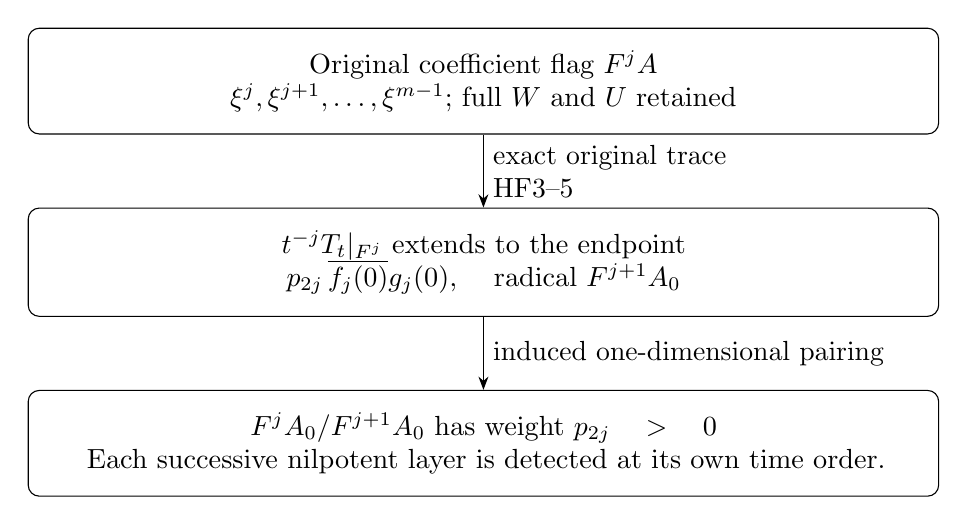
\begin{tikzpicture}[>=Stealth,
 box/.style={draw,rounded corners,align=center,text width=11cm,inner sep=8pt}]
\node[box] (a) at (0,0)
 {Original coefficient flag $F^jA$\\
 $\xi^j,\xi^{j+1},\ldots,\xi^{m-1}$; full $W$ and $U$ retained};
\node[box] (b) at (0,-2.3)
 {$t^{-j}T_t|_{F^j}$ extends to the endpoint\\
 $p_{2j}\,\overline{f_j(0)}g_j(0)$,
 \quad radical $F^{j+1}A_0$};
\draw[->] (a)--node[right,align=left]
 {exact original trace\\HF3--5}(b);
\node[box] (c) at (0,-4.6)
 {$F^jA_0/F^{j+1}A_0$ has weight $p_{2j}>0$\\
 Each successive nilpotent layer is detected at its own time order.};
\draw[->] (b)--node[right]{induced one-dimensional pairing}(c);
\end{tikzpicture}
\par\vspace{6mm}
\renewcommand{\arraystretch}{1.4}
\begin{tabular}{ccl}
\toprule
Multiplicity&First time order&$T_t(\beta v^{m-1},\beta v^{m-1})/|\beta|^2$\\
\midrule
$2$&$t$&$t+4dt^2+O(t^3)$\\
$3$&$t^2$&$\frac92t^2+36dt^3+O(t^4)$\\
$4$&$t^3$&$\frac{81}2t^3+(486d-18c^2)t^4+O(t^5)$\\
\bottomrule
\end{tabular}
\caption{The original endpoint nilpotent flag and its evaluated heat
responses, HF1--11. The coordinate remains $v=i\xi/2$ and the
arithmetic coefficients remain $c=a_{m+1}/a_m$, $d=a_{m+2}/a_m$.
The table describes the exact formulas for those orders, without
asserting that a multiple zeta zero exists. The source heat convention
is Rodgers--Tao v5; the original reflected arithmetic trace is the
Connes--Consani receiver cited at the start of this section.}
\end{figure}

\section{The original logarithmic connection and its synchronized support decomposition}
\label{sec:heat-lattice-receiver}

Use the complete convergent substitution proved in the preceding
integral-lattice derivation: $\xi=F(t,y)=y+tB(t,y)$, from
\[
 A=\mathcal O[\xi]/W(t,\xi)
       \xrightarrow[\xi\mapsto F(t,y)]{\ \sim\ }
 A_H=\mathcal O[y]/P_m(t,y),\qquad
 P_m(t,y)=\prod_{a=1}^r(y^2-b_a^2t)\,y^\varepsilon,
 \tag{HL1}
\]
where $\mathcal O=\mathbb C\{t\}$, $r=\lfloor m/2\rfloor$,
$\varepsilon=m-2r$, and $b_a$ are the positive roots of HF2.
The full actual coefficients remain in $F$ and its inverse.
Let $T$ take a coefficient column in the original $\xi$ basis to
its coefficient column in the $y$ basis. The proved substitution
has $T\in\mathrm{GL}_m(\mathcal O)$ and $T(0)=I$.
The calculations below give the exact receivers of this isomorphism;
they do not substitute $P_m$ for the original arithmetic function.

\paragraph{HL1. The connection on the original coefficient lattice.}
Weighted homogeneity gives
$2t\partial_tP_m+y\partial_yP_m=mP_m$.
Consequently on the generic fibre the original root connection,
whose horizontal coordinates are branch evaluations, is
$\partial_t+(y/(2t))\partial_y$ in $A_H$.
On its ordered power basis it has matrix
$D/(2t)$, where $D=\operatorname{diag}(0,1,\ldots,m-1)$.
The chain rule for the exact coefficient map $T$ therefore proves
\[
 \Gamma_A=T^{-1}\left(\frac{D}{2t}T+T'\right),
 \qquad t\nabla A\subseteq A,
 \qquad \operatorname{Res}_{t=0}\nabla\big|_A=\frac D2.
 \tag{HL2}
\]
Indeed for an original column $f$, the transformed covariant
derivative is $(Tf)'+(D/(2t))Tf$; multiplying by $T^{-1}$ gives
HL2. Since $T$ and its inverse are analytic and $T(0)=I$, the
matrix has only a simple pole and the stated residue.
This is the actual original connection, including the unit term
$2U_\xi/U$ proved in HH8; the equality follows from their identical
branch-evaluation derivatives under HL1.

The original monodromy is thus the regular algebra involution
\[
 M_A=T^{-1}\operatorname{diag}((-1)^k)_{k=0}^{m-1}T,
       \qquad M_A(A)=A.
 \tag{HL3}
\]
It is the conjugate of $y\mapsto-y$, so it squares to the identity
and preserves the unit and product. At the endpoint it sends
$\xi^k\mapsto(-1)^k\xi^k$ with every nilpotent retained.

\paragraph{HL2. The conductor index is the exact residue shift.}
Let $B$ be the integral closure of HC5, and use its ordered
component basis $1,u_a$ with $u_a^2=t$, and the central $1$ when
$\varepsilon=1$. Its connection residue has $r+\varepsilon$
zeros and $r$ copies of $1/2$. The original inclusion is the full
matrix $J=C(t)\operatorname{diag}(t^{\lfloor k/2\rfloor})$ of HC7,
with $C(t)$ analytic and invertible. The same chain rule gives
\[
 \Gamma_A=J^{-1}(\Gamma_BJ+J'),\qquad
 \operatorname{Tr}\Gamma_A-\operatorname{Tr}\Gamma_B
    =\frac d{dt}\log\det J
    =\frac{\delta}{t}+\frac d{dt}\log\det C(t),
 \tag{HL4}
\]
where
\[
 \delta=\sum_{k=0}^{m-1}\lfloor k/2\rfloor
   =\left\lfloor\frac{(m-1)^2}{4}\right\rfloor
   =\operatorname{length}_{\mathcal O}(B/A).
 \tag{HL5}
\]
The logarithmic derivatives in HL4 denote $f'/f$ for the displayed
nonzero determinants, so they require no choice of logarithm.
The trace residue difference also equals
$\sum_{k=0}^{m-1}k/2-r/2=m(m-1)/4-r/2=\delta$.
Thus the full coefficient lattice and the integral closure differ
by the precisely evaluated integer parts of their connection
exponents. The analytic determinant unit is retained in HL4.

\paragraph{HL3. Fixed and anti-fixed amplitudes.}
Define $Q(t,z)=\prod_{a=1}^r(z-b_a^2t)$, with empty product $1$.
The coefficient parity of $P_m(t,y)$ proves the following exact
module decomposition under HL1:
\[
 \begin{array}{c|c|c}
 & A^+=\ker(M_A-I)&A^-=\ker(M_A+I)\\ \hline
 m=2r&\mathcal O[z]/Q(t,z)&y\,\mathcal O[z]/Q(t,z)\\
 m=2r+1&\mathcal O[z]/(zQ(t,z))&y\,\mathcal O[z]/Q(t,z).
 \end{array}
 \tag{HL6}
\]
Here $z=y^2$ and the notation in the two columns is carried back
to the original coordinate by the inverse of HL1. The left column
is a subalgebra. The right column is a module, with its products
landing in the left column; it is not asserted to be a subalgebra.
For even $m$, the relation is exactly $Q(t,y^2)=0$; separating
even and odd coefficients gives both columns. For odd $m$, the
relation $yQ(t,y^2)=0$ gives $zQ(t,z)=0$ in even degree and
$Q(t,z)=0$ in odd degree. The bases $1,y,\ldots,y^{m-1}$ show
that there are no further relations. This proves HL6 including
the empty odd column at $m=1$.

For real $t$, the substitution coefficients are real, by uniqueness
of interpolation from the real Taylor coefficients of $H_t$.
Thus $M_A$ commutes with reflection and preserves $T_t$.
If $a\in A^+$, $b\in A^-$, then
$T_t(a,b)=T_t(M_Aa,M_Ab)=-T_t(a,b)$, so
\[
 T_t(A^+,A^-)=0.
 \tag{HL7}
\]
This holds as an identity of the full analytic Gram matrices,
including the endpoint. The endpoint socle $\mathbb C\xi^{m-1}$
lies in the plus column for odd $m$ and in the minus column for
even $m$. Its deformed trace sign from HF10 at negative $t$ is
therefore exactly its monodromy sign. Its actual endpoint trace
is still zero when $m\ge2$.

\paragraph{HL4. The supported projections have an exact common residue.}
The amplitude projections $E_\pm=(I\pm M_A)/2$ obey
$E_+E_-=0$ and $E_++E_-=I$. Lift them to the full supported
$G_L(\mathcal O)$-semimodule $G_L(A)$ by
\[
 \widehat E_\pm(a,\lambda)=(E_\pm a,\lambda),
       \qquad \kappa(a,\lambda)=(0,\lambda).
 \tag{HL8}
\]
Only zero amplitude is allowed below the top support, as in the
original definition. These formulas are consequently well-defined
and additive, and they commute with every scalar in
$G_L(\mathcal O)$: amplitude linearity and the meet of supports
give the assertion directly. Exact composition now gives
\[
 \widehat E_\pm^2=\widehat E_\pm,\qquad
 \widehat E_++\widehat E_-=I,\qquad
 \boxed{\widehat E_+\widehat E_-
            =\widehat E_-\widehat E_+=\kappa.}
 \tag{HL9}
\]
The last map preserves the original support while its amplitude
vanishes. For top-supported input it returns $e$, and for a zero
label $z_\lambda$ it returns that same label. It returns $\tau$
only at $\tau$. Thus no disappearance of a supported component
is inferred from the ordinary amplitude product of projections.

The exact inverse construction is the synchronized module
\[
 \mathcal S=\{((a_+,\lambda),(a_-,\lambda)):
       a_\pm\in A^\pm,\text{ with the allowed original supports}\}.
 \tag{HL10}
\]
The map $G_L(A)\to\mathcal S$ is
$(a,\lambda)\mapsto((E_+a,\lambda),(E_-a,\lambda))$;
its inverse is $((a_+,\lambda),(a_-,\lambda))\mapsto
(a_++a_-,\lambda)$. Addition uses joins of the common supports.
Equip $\mathcal S$ with multiplication
\[
 ((a_+,a_-),\lambda)((b_+,b_-),\mu)
   =((a_+b_++a_-b_-,\ a_+b_-+a_-b_+),\lambda\wedge\mu).
 \tag{HL11}
\]
The parity product rules from HL6 show that both components land
in the stated modules. Expansion of $(a_++a_-)(b_++b_-)$ proves
that the displayed inverse preserves multiplication and the unit.
It is therefore an exact semiring isomorphism for HL11, in
addition to its semimodule isomorphism. The whole lattice $L$
is shared, never replaced by two independent copies or by a
Boolean scalar. Both the amplitude map and the support map commute
with this isomorphism. This is the supported receiver of the
regular original collision monodromy.

\paragraph{HL5. The positive eight-state collision algebra and its full support.}
The same proved $C_2$-projection construction has a concrete receiver
for the new eight-state intake. Use its original critical fibre,
with all coordinates retained:
\[
 \mathcal A_c=\mathcal L\times K_-\times K_\infty,\qquad
 \mathcal L=\mathbb C[T]/T^4,\quad
 K_-=\mathbb C[S]/(S^2-9),\quad
 K_\infty=\mathbb C[\Theta]/(\Theta^2+1).
 \tag{HL12}
\]
The original collision coordinate is $\epsilon=T^2/6$.
These are the original chart and collision formulas of
\href{https://github.com/KokunoYumeto/zeta-function-research-reader/blob/64a77de144720ea9e07943d6ed6f63a178d462cf/workbenches/splitzero-tandem/branches/tau-zero-prime-positivity/EIGHT_STATE_HEAT_COMPARISON.md}{\emph{The signed eight-state completion and its exact heat receivers}}.
The computations required here are given in full below.
The fibre involution used here conjugates coefficients and sends
$T,S,\Theta$ to their negatives. It is the conjugate-deck involution.
The native target-reflection involution instead maps this target
to its reflected target, as proved by that source's equations
ESH17--18; no self-involution of a single moving fibre is inferred
from that separate map.

Writing $x=(\ell,c+dS,\eta_0+\eta_1\Theta)$, multiplication
in the three unchanged power bases gives
\[
 Q_c(x)=4|\ell(0)|^2+2|c|^2-18|d|^2
                         +2|\eta_0|^2+2|\eta_1|^2.
 \tag{HL13}
\]
Indeed the trace on $\mathcal L$ is four times the constant
coefficient; every higher multiplication power of $T$ has zero
diagonal. In $K_-$, $S^\#S=-9$ and the trace of $1$ is two.
In $K_\infty$, $\Theta^\#\Theta=1$ and the same trace is two.
All cross terms have zero scalar coefficient. This proves the
whole sesquilinear form by polarization, with inertia $(4,1,3)$.

Define the actual algebra involution
$\sigma_c(\ell,c+dS,z)=(\ell,c-dS,z)$.
Its fixed subalgebra and its anti-fixed module are
\[
 \mathcal A_c^+=\mathcal L\times\mathbb C\times K_\infty,
 \qquad \mathcal A_c^-=\{(0,dS,0):d\in\mathbb C\}.
 \tag{HL14}
\]
It commutes with the displayed conjugate-deck involution.
The group-algebra homomorphism
$\mathbb C[C_2]\to\operatorname{End}_{\mathbb C}(\mathcal A_c)$,
whose generator maps to $\sigma_c$, sends $(1\pm g)/2$ to
the two projections in HL14. The analogous homomorphism for
the original heat algebra sends $g$ to $M_A$. These give the
exact common domain and the two concrete receivers of HL8--11;
they do not identify their distinct coefficient algebras.

The fixed projection $E_c=(I+\sigma_c)/2$ satisfies the exact
identities
\[
 \begin{gathered}
 Q_c(x)=Q_c(E_cx)-18|d|^2,\qquad
 \operatorname{inertia}(Q_c|_{\mathcal A_c^+})=(4,0,3),\\
 E_c(xy)-E_c(x)E_c(y)
      =(0,9d_xd_y,0).
 \end{gathered}
 \tag{HL15}
\]
The product formula follows by expanding
$(c_x+d_xS)(c_y+d_yS)$ and retaining $S^2=9$.
It evaluates the complete multiplicative defect of this particular
positive projection. The length-four local algebra is unchanged.
Its relative trace to $\mathbb C[\epsilon]/\epsilon^2$ still sends
$T^\#T=-6\epsilon$ to $-12\epsilon$, whereas the scalar trace
sends it to zero. Both maps and the nonzero relative value follow
from the free relative basis $(1,T)$.

The fixed algebra has dimension seven. A nonnegative subspace
for an inertia-$(4,1,3)$ form has dimension at most seven:
modulo its three-dimensional radical the projection of a
nonnegative subspace to the positive four-space is injective,
since its kernel would be a nonzero negative vector.
Thus this fixed subalgebra reaches that bound. It is the unique
largest nonnegative subalgebra containing the complete local and
infinity factors and their central units: in the remaining
$K_-\simeq\mathbb C^2$, a unital subalgebra containing unequal
coordinates contains both point idempotents by linear interpolation,
and then contains the whole indefinite factor. Its only
nonnegative unital alternative is the diagonal copy of $\mathbb C$.

Applying HL8--11 to $\sigma_c$ proves the full supported
projection formula, with the same $\kappa$ and every original
label. The inclusion $G_L(\mathcal A_c^+)\hookrightarrow
G_L(\mathcal A_c)$ is a unital semiring map. On arithmetic
prime spectra its contravariant map identifies the two reduced
$S=\pm3$ points and preserves the local collision point and
both infinity points. This follows from the factorwise
inclusions $\mathbb C\hookrightarrow\mathbb C^2$ and the two
identity maps in HL14. On support primes it is the identity:
an ideal determined by a lattice prime pulls back to the same
lattice prime, since every label is fixed. Hence the exact
full support spectrum map is also evaluated. This positive
subalgebra changes the two reduced $S$ directions and retains
the complete infinitesimal and its relative trace.

\clearpage
\end{document}
